\documentclass[11pt,letterpaper]{article}

%\usepackage{fontspec}
%\usepackage[utf8]{inputenc}
\usepackage{textcomp,marvosym}
\usepackage{amsmath,amssymb}
\usepackage[normalem]{ulem}
\usepackage[left]{lineno}
\usepackage{changepage}
\usepackage{sidecap}
\usepackage{rotating}
\usepackage{color}
\usepackage{natbib}
\usepackage{setspace}
\usepackage{}
\usepackage{fancyhdr}
\usepackage{graphicx}
\usepackage{xspace}
\usepackage{threeparttable}
\usepackage{color,colortbl}
\usepackage{url}
%\usepackage[hidelinks]{hyperref}
\urlstyle{same}
\doublespacing

\raggedright
\textwidth = 6.5 in
\textheight = 8.25 in
\oddsidemargin = 0.0 in
\evensidemargin = 0.0 in
\topmargin = 0.0 in
\headheight = 0.0 in
\headsep = 0.5 in
\parskip = 0.1 in
\parindent = 0.1in

% Bold the 'Figure #' in the caption and separate it from the title/caption with a period
% Captions will be left justified
\usepackage[aboveskip=1pt,labelfont=bf,labelsep=period,justification=raggedright,singlelinecheck=off]{caption}

% Remove brackets from numbering in List of References
%\makeatletter
%\renewcommand{\@biblabel}[1]{\quad#1.}
%\makeatother

% Self defined commands
\newcommand{\degreesC}{\textdegree C\xspace}
\newcommand{\degrees}{\textdegree\xspace}
\newcommand{\dC}{$\delta^{13}$C\xspace}
\newcommand{\dO}{$\delta^{18}$O\xspace}
\newcommand{\SrSr}{$^{87}$Sr/$^{86}$Sr\xspace}
\newcommand{\permil}{\textperthousand\xspace}
\newcommand{\UPb}{$^{206}$Pb/$^{238}$U\xspace}
\newcommand{\pCOtwo}{\textit{p}CO$_{2}$\xspace}
\newcommand{\COtwo}{CO$_{2}$\xspace}
%

\setcounter{figure}{0}
\renewcommand{\thefigure}{SI\arabic{figure}}
\setcounter{table}{0}
\renewcommand{\thetable}{SI\arabic{table}}

\definecolor{Yellow}{rgb}{1,1,0.35}
%

\pagestyle{myheadings}
\pagestyle{fancy}
\fancyhf{}
\lhead{Park et al., in preparation}
\rhead{\thepage}

\begin{document}

\begin{flushleft}
{\Large \textbf{Supplementary Information for ``Emergence of Indonesia and New Guinea as a driver for Neogene cooling''}}

Yuem Park\textsuperscript{1},
Nicholas L. Swanson-Hysell\textsuperscript{1},
Pierre Maffre\textsuperscript{1},
Francis A. Macdonald\textsuperscript{2},
Eliel A. Anttila\textsuperscript{2},
Yves Godd\'eris\textsuperscript{3}

\bigskip
\textsuperscript{1} Department of Earth and Planetary Science, University of California, Berkeley, CA, USA

\textsuperscript{2} Department of Earth Science, University of California, Santa Barbara, CA, USA

\textsuperscript{3} G\'eosciences Environnement Toulouse, CNRS--Universit\'e Paul Sabatier - IRD, Toulouse, France

\bigskip

\end{flushleft}

\linenumbers

These supplementary information materials provide details on the model framework used in this study. Python code used for this study can be found at: \url{https://github.com/Swanson-Hysell-Group/XXX}.

\section*{Silicate Weathering Component}

\begin{SCfigure}[0.6][h!]
\begin{center}
	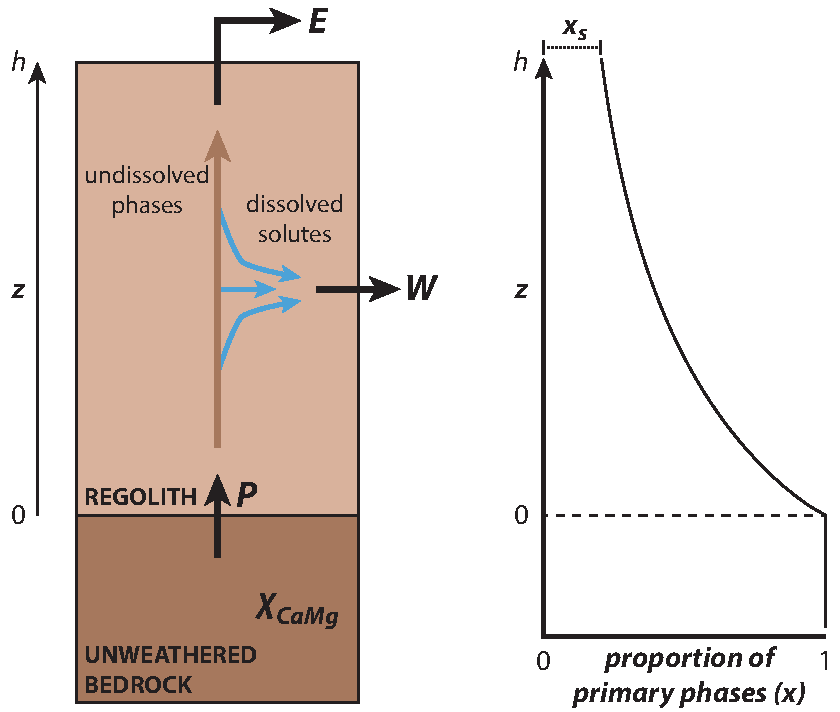
\includegraphics[width=0.6\textwidth]{../Figures/regolith_schematic.pdf}
	\caption{A schematic representation of the silicate weathering component of GEOCLIM in a single profile at steady-state. A rock particle leaves the unweathered bedrock with production rate $P$, and transits vertically through a regolith of height $h$. Regolith production and physical erosion ($E$) are equal at steady-state. As the particle transits upwards, some fraction of the primary phases ($x$) are chemically weathered ($W$) with the flux of Ca and Mg corresponding to that weathering rate multiplied by the concentration of Ca+Mg in unweathered bedrock ($\chi_{CaMg}$).}
	\label{fig:regolith_schematic}
\end{center}
\end{SCfigure}

The silicate weathering component of the GEOCLIM model implements the model of \cite{Gabet2009a} for the development of a chemically weathered profile. We refer to this chemically weathered profile as regolith where the base of the regolith is the contact with unweathered bedrock. In the model of \citet{Gabet2009a}, material enters the regolith and leaves either as a solute through chemical weathering as a particle transit through the regolith or as a physically weathered particle once it reaches the top. We use the DynSoil implementation of the \cite{Gabet2009a} model which integrates a climatic dependence on the chemical weathering that occurs within the regolith using the formulation of \cite{West2012a}. The transient time-varying versions of this regolith model is described by the following system of three equations which form the basis of DynSoil:

\begin{equation}
    \frac{dh}{dt} = P - E
    \label{eq:1}
\end{equation}

\begin{equation}
    \frac{\partial x}{\partial t} = -P \frac{\partial x}{\partial z} - K \tau^{\sigma}x
    \label{eq:2}
\end{equation}

\begin{equation}
    \frac{\partial \tau}{\partial t} = -P \frac{\partial \tau}{\partial z} + 1
    \label{eq:3}
\end{equation}

\noindent
Equation \ref{eq:1} is a statement of material conservation, where $h$ is the total height of the regolith (m), $t$ is the time in the model (yr), $P$ is the regolith production rate (m/yr), and $E$ is the physical erosion rate (m/yr). Equation \ref{eq:2} describes how the residual fraction of weatherable phases ($x$, unitless) changes as a function of time ($t$, yr) and depth (where $z$ is the height above the base of the regolith; m). $K \tau^{\sigma}$ is the dissolution rate constant, which depends on the local climate (captured by $K$, yr$^{-1-\sigma}$) and the time that a given rock particle has spent in the regolith ($\tau$, yr) to some power $\sigma$ (unitless) which implements a time-dependence. Equation \ref{eq:3} describes how the time that a given rock particle has spent in the regolith changes as time in the model progresses.

The net weathering rate in the regolith column ($W$, m/yr) can then be calculated with:

\begin{equation}
    W = \int_{0}^{h} K \tau^{\sigma} x\;dz
    \label{eq:4}
\end{equation}

The regolith production rate can be expressed as the product of the optimal production rate ($P_{0}$) and the soil production function ($f(h)$):

\begin{equation}
    P = P_{0}\;f(h)
    \label{eq:5}
\end{equation}

\begin{equation}
    P_{0} = k_{rp}\;q\;e^{-\frac{E_{a}}{R}\left(\frac{1}{T}-\frac{1}{T_{0}}\right)}
    \label{eq:6}
\end{equation}

\begin{equation}
    f(h) = e^{-\frac{-h}{d_{0}}}
    \label{eq:7}
\end{equation}

\noindent
$P_{0}$ is the `optimal' regolith production rate (m/yr), which is defined to be the regolith production rate when there is no overlying regolith. In Equation \ref{eq:6}, we parameterize this value using the model of \citet{Carretier2014a}, where $k_{rp}$ is a proportionality constant (unitless), $q$ is the runoff (m/yr), $E_{a}$ is the activation energy (J/K/mol), $R$ is the universal gas constant (J/mol), $T$ is the temperature (K), and $T_{0}$ is the reference temperature (K). $f(h)$ is the soil production function (unitless), which describes how regolith production decreases as the thickness of the regolith increases. It takes an exponential form as is commonly applied in the literature (e.g. \citealp{Gabet2009a}). In Equation \ref{eq:7}, we follow \citet{Heimsath1997a}, where $d_{0}$ is a reference regolith thickness (m).

Our implementation of the erosion rate follows one of the approaches taken in \citet{Godderis2017c} and \citet{Maffre2018a}, where it is parameterized based on runoff and slope ($s$; m/m):

\begin{equation}
    E = k_{e}\;q^{m}\;s^{n}
    \label{eq:8}
\end{equation}

\noindent
$k_{e}$ is a proportionality constant ((m/yr)$^{1-m}$) and $m$ and $n$ are adjustable exponents that are kept as 0.5 and 1 as in \citet{Maffre2018a}. This formulation is similar to the large-scale BQART model of \citet{Syvitski2007a}, but without a temperature dependence and the replacement of elevation with slope, resulting in functional form that more closely resembles the stream power law \citep{Davy2000a}. This form and these exponent values are supported by various compilations (e.g. \citealp{Lague2014a}) although \citet{Lague2014a} also suggests that there is variability in the proportionality constant that is difficult to capture at a global scale.

The $K$ in the dissolution rate constant in Equation \ref{eq:2} describes the dependence of the chemical weathering on climate:

\begin{equation}
    K = k_{d}\left(1-e^{-k_{w}q}\right)e^{-\frac{E_{a}}{R}\left(\frac{1}{T}-\frac{1}{T_{0}}\right)}
    \label{eq:9}
\end{equation}

\noindent
Equation \ref{eq:9} is an empirical simplification of mineral dissolution rates derived from kinetic theory and laboratory experiments \citep{West2012a}, where $k_{d}$ is a proportionality constant that modifies the dependence of dissolution rate on runoff and temperature (yr$^{-1-\sigma}$), and $k_{w}$ is a proportionality constant that modifies the dependence of dissolution rate on runoff (yr/m).

In this study, we are interested in obtaining the steady-state solution rather than the transient time-varying solution. The steady-state solution for DynSoil can be calculated analytically by setting the time derivatives equal to zero resulting in the following set of equations:

\begin{equation}\label{eq:dynsoil_ss}
\left\{\ 
\begin{aligned}
& h   \ =\    \max\left(  \;  0  \;,\;  d_o \log\left(\frac{P_o}{E}\right)  \right)                                                 \\
& x(z)      \ =\   \exp\left(   - \frac{K}{\sigma+1}  \left(\frac{z}{E}\right)^{\sigma+1}   \right)   \\
& W        \ =\   (1-x(h)) \, E  \ =\   (1-x_s) \, E                                                                         \\
\end{aligned}
\right.
\end{equation}

\noindent
$x(z)$ gives the curve of primary phases varying with height upward from the base of the regolith as shown in Figure \ref{fig:regolith_schematic}. Setting $z$ equal to regolith thickness ($h$) gives $x_s$ which is the proportion of primary phases remaining at the top of the column of regolith. This value controls the overall integrated chemical weathering rate out of the regolith.

\section*{Implementation of Lithology}

\begin{table}[h!]
\begin{center}
\resizebox{0.7\textwidth}{!}{
    \begin{tabular}{cclcl}
    \textbf{GLiM} & \textbf{GLiM} & \textbf{GLiM} & \textbf{GEOCLIM} & \textbf{GEOCLIM}\\
    \textbf{ID} & \textbf{code} & \textbf{classification} & \textbf{ID} & \textbf{classification}\\
    &&&& \\
    \hline
    &&&& \\
    1 & su & unconsolidated sediments & 6 & sediments \\
    2 & vb & basic volcanic rocks & 4 & mafics \\
    3 & ss & siliciclastic sedimentary rocks & 6 & sediments \\
    4 & pb & basic plutonic rocks & 4 & mafics \\
    5 & sm & mixed sedimentary rocks & 6 & sediments \\
    6 & sc & carbonate sedimentary rocks & 5 & carbonates \\
    7 & va & acid volcanic rocks & 2 & felsics \\
    8 & mt & metamorphics & 1 & metamorphics \\
    9 & pa & acid plutonic rocks & 2 & felsics \\
    10 & vi & intermediate volcanic rocks & 3 & intermediates \\
    11 & wb & water bodies & 0 & water/ice \\
    12 & py & pyroclastics & 2 & felsics \\
    13 & pi & intermediate plutonic rocks & 3 & intermediates \\
    14 & ev & evaporites & 5 & carbonates \\
    15 & nd & no data & 1 & metamorphics \\
    16 & ig & ice and glaciers & 0 & water/ice \\
    \end{tabular}
}
\vspace{10pt}
\caption{Grouping of 16 lithologic categories in GLiM \citep{Hartmann2012a} to 6 broader categories for GEOCLIM.}
\label{tab:GLiM_to_GEOCLIM}
\end{center}
\end{table}

\begin{figure}[h!]
    \centering
    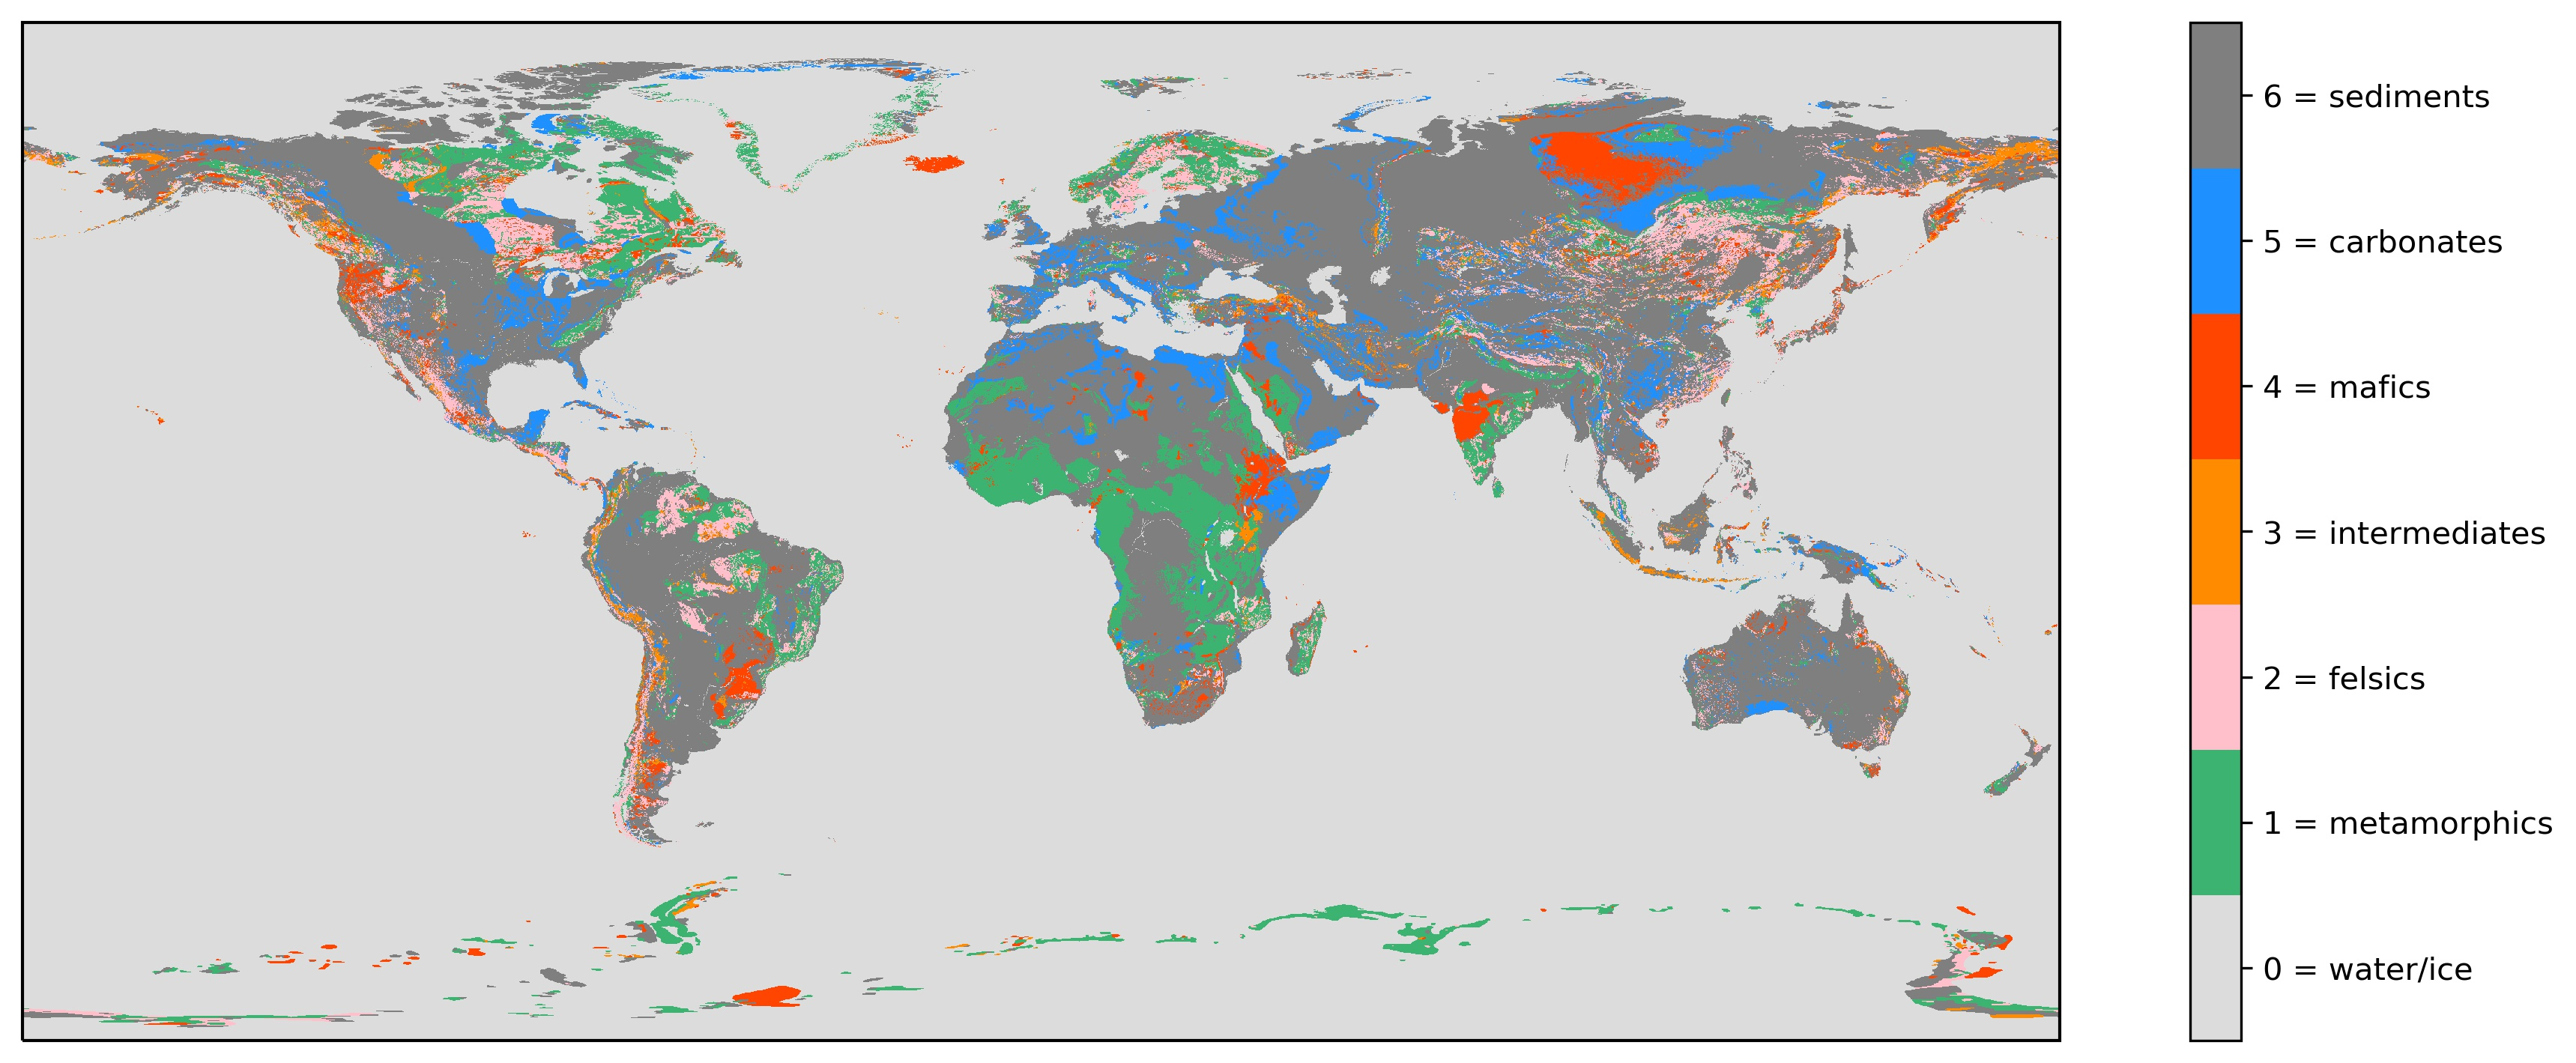
\includegraphics[width=1\textwidth]{Manuscript/Figures/world_lithology.jpg}
    \caption{Distribution of lithologies at 0.1\degrees $\times$ 0.1\degrees resolution used in GEOCLIM.}
    \label{fig:world_lithology}
\end{figure}

To calculate the flux of Ca and Mg associated with chemical weathering, we need to assign the concentration of Ca and Mg ($\chi_{CaMg}$) within the unweathered bedrock (Fig. \ref{fig:regolith_schematic}). Previous implementations of GEOCLIM have taken bulk continental crust values across all land. Given that the hypothesis we seek to test involves the varying concentration of cations in different lithologies, we have implemented a lithologically resolved version of the model.

The spatial distribution of lithologies is sourced from the global lithologic map (GLiM) of \citet{Hartmann2012a}. The raw data takes the form of polygon vectors, where each polygon is assigned one of 16 lithologic categories. We first group these 16 categories into 6 broader categories (metamorphic, felsic, intermediate, mafic, carbonate, and siliciclastic sediment; Table \ref{tab:GLiM_to_GEOCLIM}). We then rasterize the polygon vectors to 0.1\degrees $\times$ 0.1\degrees resolution, where each pixel is assigned the lithologic category of the polygon that covers the greatest area in that pixel (i.e. the `mode lithology'; Fig. \ref{fig:world_lithology}). However, to improve the computing time of GEOCLIM, we decrease the resolution of the raster to 0.5\degrees $\times$ 0.5\degrees. To do so, a 3-dimensional 720 $\times$ 360 $\times$ 7 matrix is created, in which the fraction of each 0.5\degrees $\times$ 0.5\degrees pixel that is covered by each of the 6 lithologic categories + water/ice is captured by the extra dimension. In this way, GEOCLIM is able to calculate the area-weighted mean Mg+Ca concentration of the surface in each 0.5\degrees $\times$ 0.5\degrees pixel.

\section*{GEOCLIM Calibration}

Experimental determinations of the activation energy ($E_a$; Equations \ref{eq:8} and \ref{eq:9}) associated with the weathering of silicate minerals are variable \citep{Brantley2003a}. However, multiple efforts to invert for $E_a$ in basaltic watersheds with varying temperature have yielded values (41.6 $\pm$ 3.2~kJ/mol in \citealp{Li2016a}; 42.3~kJ/mol in \citealp{Dessert2001a}) that are consistent with the lower end of activation energies of Ca+Mg bearing minerals in laboratory experiments such as that for diopside (40.5 $\pm$ 1.7~kJ/mol; \citealp{Knauss1993a}) and for labradorite (42.1~kJ/mol; \citealp{Carroll2005a}. We use the value of 42~kJ/mol in our model runs.

However, as discussed in the main text, $k_{d}$ (Equation \ref{eq:9}), $k_{w}$ (Equation \ref{eq:9}), $\sigma$ (Equation \ref{eq:4}), and $k_{rp}$ (Equation \ref{eq:8}) are poorly constrained. Furthermore, the Ca+Mg concentrations of metamorphic and siliciclastic sediment grid cells are also difficult to define. We therefore allow these parameters to vary within reasonable bounds during the calibration stage of GEOCLIM (Table \ref{tab:parameter_combinations}).

\begin{table}[h!]
\begin{center}
\resizebox{0.6\textwidth}{!}{
    \begin{tabular}{cccccc}
    \textbf{$k_{d}$} & \textbf{$k_{w}$} & \textbf{$\sigma$} & \textbf{$k_{rp}$} & \textbf{metamorphic$_{\text{Ca}+\text{Mg}}$} & \textbf{sediment$_{\text{Ca}+\text{Mg}}$}\\
    unitless & unitless & unitless & unitless & mol/m$^{3}$ & mol/m$^{3}$ \\
    &&&&& \\
    \hline
    &&&&& \\
    1$\times$10$^{-5}$ & 1$\times$10$^{-3}$ & -0.4 & 1.2$\times$10$^{-3}$ & 1500 & 500 \\
    2$\times$10$^{-5}$ & 2$\times$10$^{-3}$ & -0.2 & 2$\times$10$^{-3}$ & 2000 & 1000 \\
    5$\times$10$^{-5}$ & 5$\times$10$^{-3}$ & -0.1 & 3$\times$10$^{-3}$ & 2500 & 1500 \\
    1$\times$10$^{-4}$ & 1$\times$10$^{-2}$ & 0 & 5$\times$10$^{-3}$ & 3000 & 2000 \\
    2$\times$10$^{-4}$ & 2$\times$10$^{-2}$ & 0.1 &  & 3500 & 2500 \\
    5$\times$10$^{-4}$ & 5$\times$10$^{-2}$ & 0.3 &  & 4000 & 3000 \\
    1$\times$10$^{-3}$ & 1$\times$10$^{-1}$ &  &  &  &  \\
    2$\times$10$^{-3}$ & 2$\times$10$^{-1}$ &  &  &  &  \\
    5$\times$10$^{-3}$ & 5$\times$10$^{-1}$ &  &  &  &  \\
    1$\times$10$^{-2}$ & 1 &  &  &  &  \\
    \end{tabular}
}
\vspace{10pt}
\caption{Values tested for poorly constrained parameters in the silicate weathering component of GEOCLIM. Every permutation of the listed values were tested (except those permutations where the Ca+Mg concentration of the sediments are higher than that of the metamorphics), resulting in 78,000 unique parameter combinations.}
\label{tab:parameter_combinations}
\end{center}
\end{table}

We then compute spatially-resolved long-term \COtwo consumption (i.e. Ca+Mg consumption) using present-day runoff, temperature, and slope fields. As described in the main text, we then sum the computed \COtwo consumption over large-scale watersheds that appear in the global compilation of \citet{Gaillardet1999a}, as well as smaller-scale watersheds of the Amazon Basin in the compilation of \citet{Moquet2011a, Moquet2016a, Moquet2018a}. 80 watersheds in total are used in this study. We then calculate the coefficient of determination ($r^{2}$) between computed and measured \COtwo consumption in each of these basins:

\begin{equation}
    r^{2} = 1 - \frac{\sum\left[ \log_{10}(M_{i}) - \log_{10}(O_{i}) \right]^{2}}{\sum\left[ \log_{10}(O_{i}) - \overline{\log_{10}(O)} \right]^{2}}
    \label{eq:10}
\end{equation}

\noindent
$M_{i}$ is the modeled \COtwo consumption over watershed $i$, $O_{i}$ is the observed \COtwo consumption over watershed $i$, and $\overline{\log_{10}(O)}$ is the mean of the log of observed \COtwo consumption over all watersheds.

% FIGURE: CO2 consumption vs r^2
% FIGURE: CO2 consumption cross plot


%% FROM MAIN TEXT
Of the various parameters used in the equations that govern the silicate weathering component of GEOCLIM (see SI), four parameters in particular are poorly constrained in the existing literature: the proportionality constant that modifies the dependence of dissolution rate on runoff and temperature ($k_{d}$), the proportionality constant that modifies the dependence of dissolution rate on runoff only ($k_{w}$), the power constant that modifies the dependence of dissolution rate on the time that a rock particle has spent in the regolith ($\sigma$), and the proportionality constant that modifies the dependence of regolith production on runoff and temperature ($k_{rp}$). As discussed above, the Ca+Mg concentrations of metamorphic and siliciclastic sediment grid cells are also difficult to define. Rather than prescribing values for these six parameters, we instead allow these parameters to vary within reasonable bounds, resulting in a total of 78,000 unique parameter combinations. For each of these combinations, we compute spatially-resolved long-term \COtwo consumption (i.e. Ca+Mg consumption) using present-day runoff, temperature, and slope fields. Following the approach of \citet{Maffre2018a}, we then sum the computed \COtwo consumption over large-scale watersheds that appear in the global compilation of \citet{Gaillardet1999a}, as well as smaller-scale watersheds of the Amazon Basin in the compilation of \citet{Moquet2011a, Moquet2016a, Moquet2018a}. We then calculate the coefficient of determination ($r^{2}$) between computed and measured \COtwo consumption in each of these basins. We eliminate all parameter combinations that result in unreasonable total global \COtwo consumption (which we define to be \textless1$\times$10$^{12}$~mol/yr or \textgreater1$\times$10$^{13}$~mol/yr) and/or result in a low $r^{2}$ (which we define to be \textless0.4). This calibration method leaves 3,339 unique parameter combinations that produce global and individual watershed \COtwo consumption fluxes that approximate those estimated in the literature for the present-day.

\section*{Climate Model}

xxx

\section*{Paleoshorelines}

xxx

\clearpage

\singlespacing

\newpage

\bibliographystyle{gsabull}
\bibliography{References}

\end{document}
